\begin{figure*}
\centering
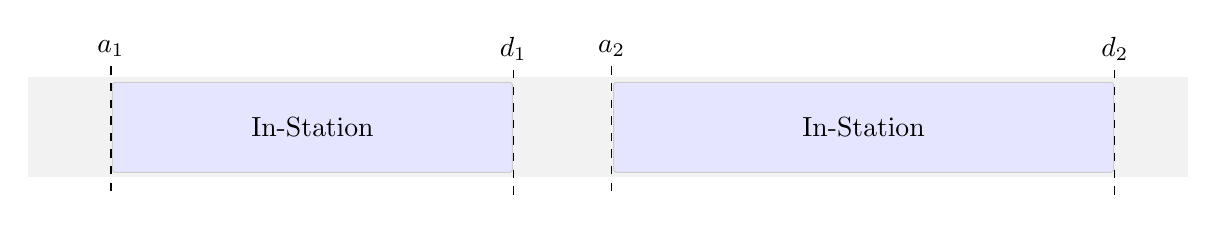
\begin{tikzpicture} 
	\node[rectangle, fill=gray!10, minimum width=5.8in, minimum height=0.5in](busAvail) at (7.75,4){}; 

	\node[rectangle, draw=blue!10!black!20, fill=blue!10, minimum width=2in, minimum height=0.45in, rounded corners=1pt](busAvail1) at (4,4){In-Station};
	\node[rectangle, draw=blue!10!black!20, fill=blue!10, minimum width=2.5in, minimum height=0.45in, rounded corners=1pt](busAvail2) at (11,4){In-Station};

	\node(firstATop) at (1.44,5){$a_1$};
	\node(firstABtm) at (1.44,3.1){};
	\draw[dashed, line width=0.5pt](firstATop) -- (firstABtm.center);
	\node(firstDTop) at (6.55,5){$d_1$};
	\node(firstDBtm) at (6.55,3.1){};
	\draw[dashed, line width=0.5pt](firstDTop) -- (firstDBtm.center);

	\node(secondATop) at (7.8,5){$a_2$};
	\node(secondABtm) at (7.8,3.1){};
	\draw[dashed, line width=0.5pt](secondATop) -- (secondABtm.center);
	\node(secondDTop) at (14.19,5){$d_2$};
	\node(secondDBtm) at (14.19,3.1){};
	\draw[dashed, line width=0.5pt](secondDTop) -- (secondDBtm.center);


\end{tikzpicture}
\caption{Bus availability}
\label{fig:busTime2}
\end{figure*}
